\documentclass[12pt]{article}
\usepackage{color}
\usepackage{tikz}
\usetikzlibrary{decorations.pathmorphing} % Añade esta línea si vas a usar decoraciones como 'snake'
\usepackage{amsmath}
\usepackage{amssymb}

\begin{document}

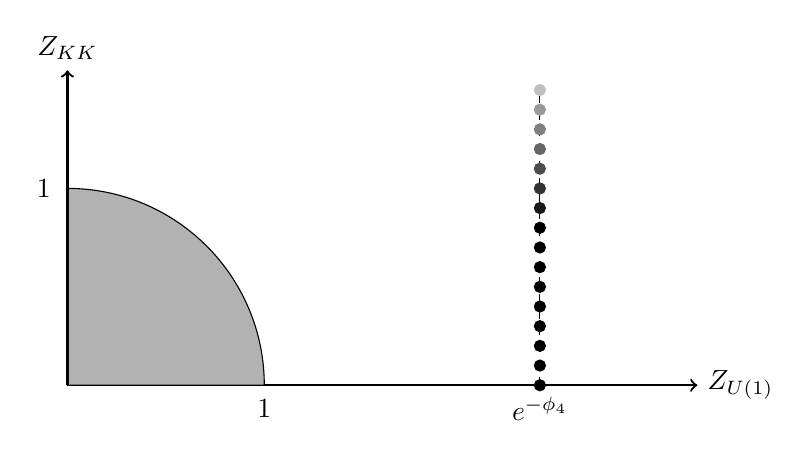
\begin{tikzpicture}
% Eje horizontal más largo
\draw[->,thick] (0,0) -- (8,0) node[right] {$Z_{U(1)}$};
% Cuarto de circunferencia de radio 2
% Cuarto de circunferencia de radio 2 pintado de gris oscuro
\filldraw[fill=gray!60] (0,0) -- (2.5,0) arc (0:90:2.5) -- cycle;
% Eje vertical más corto
\draw[->,thick] (0,0) -- (0,4) node[above] {$Z_{KK}$};
\draw[-,dashed] (6,0) -- (6,3.8);

\node at (6,-0.3) {$e^{-\phi_4}$};
\filldraw[black] (6,1.25) circle (2pt);
\filldraw[black] (6,1) circle (2pt);
\filldraw[black] (6,0.75) circle (2pt);
\filldraw[black] (6,0.5) circle (2pt);
\filldraw[black] (6,0.25) circle (2pt);
\filldraw[black] (6,0) circle (2pt);
\filldraw[black] (6,1.5) circle (2pt);
\filldraw[black] (6,1.75) circle (2pt);
\filldraw[black] (6,2) circle (2pt);
\filldraw[black!90] (6,2.25) circle (2pt);
\filldraw[black!80] (6,2.5) circle (2pt);
\filldraw[black!70] (6,2.75) circle (2pt);
\filldraw[black!60] (6,3) circle (2pt);
\filldraw[black!50] (6,3.25) circle (2pt);
\filldraw[black!40] (6,3.5) circle (2pt);
\filldraw[black!25] (6,3.75) circle (2pt);


% Etiquetas de los ejes
\node at (2.5,-0.3) {$1$};
\node at (-0.3,2.5) {$1$};
\end{tikzpicture}

\end{document}